\documentclass[ignorenonframetext,notes, 10pt, aspectratio=169]{beamer}

\usepackage{preamble_slides}


\title{\textbf{\Large{Introduction to git for social science students}}}
\providecommand{\subtitle}[1]{}
\subtitle{(not software developers)}
\author{Shiro Kuriwaki}
\date{March 5, 2019}

\begin{document}

\begin{frame}{Setup}
\begin{columns}[T]
\begin{column}{0.6\textwidth}
\begin{wideenumerate}
\item Go to \url{www.github.com} and make a free account
% https://happygitwithr.com/github-acct.html#username-advice
\item Make sure you have a recent version (v1.1 or later) of RStudio \url{https://www.rstudio.com/products/rstudio/download/\#download}
\item Keep \url{www.happygitwithr.com} open
\item Download these slides via: \url{https://github.com/kuriwaki/github-demo/raw/master/presentation-slides/kuriwaki_github.pdf}
\end{wideenumerate}
\end{column}
\begin{column}{0.4\textwidth}
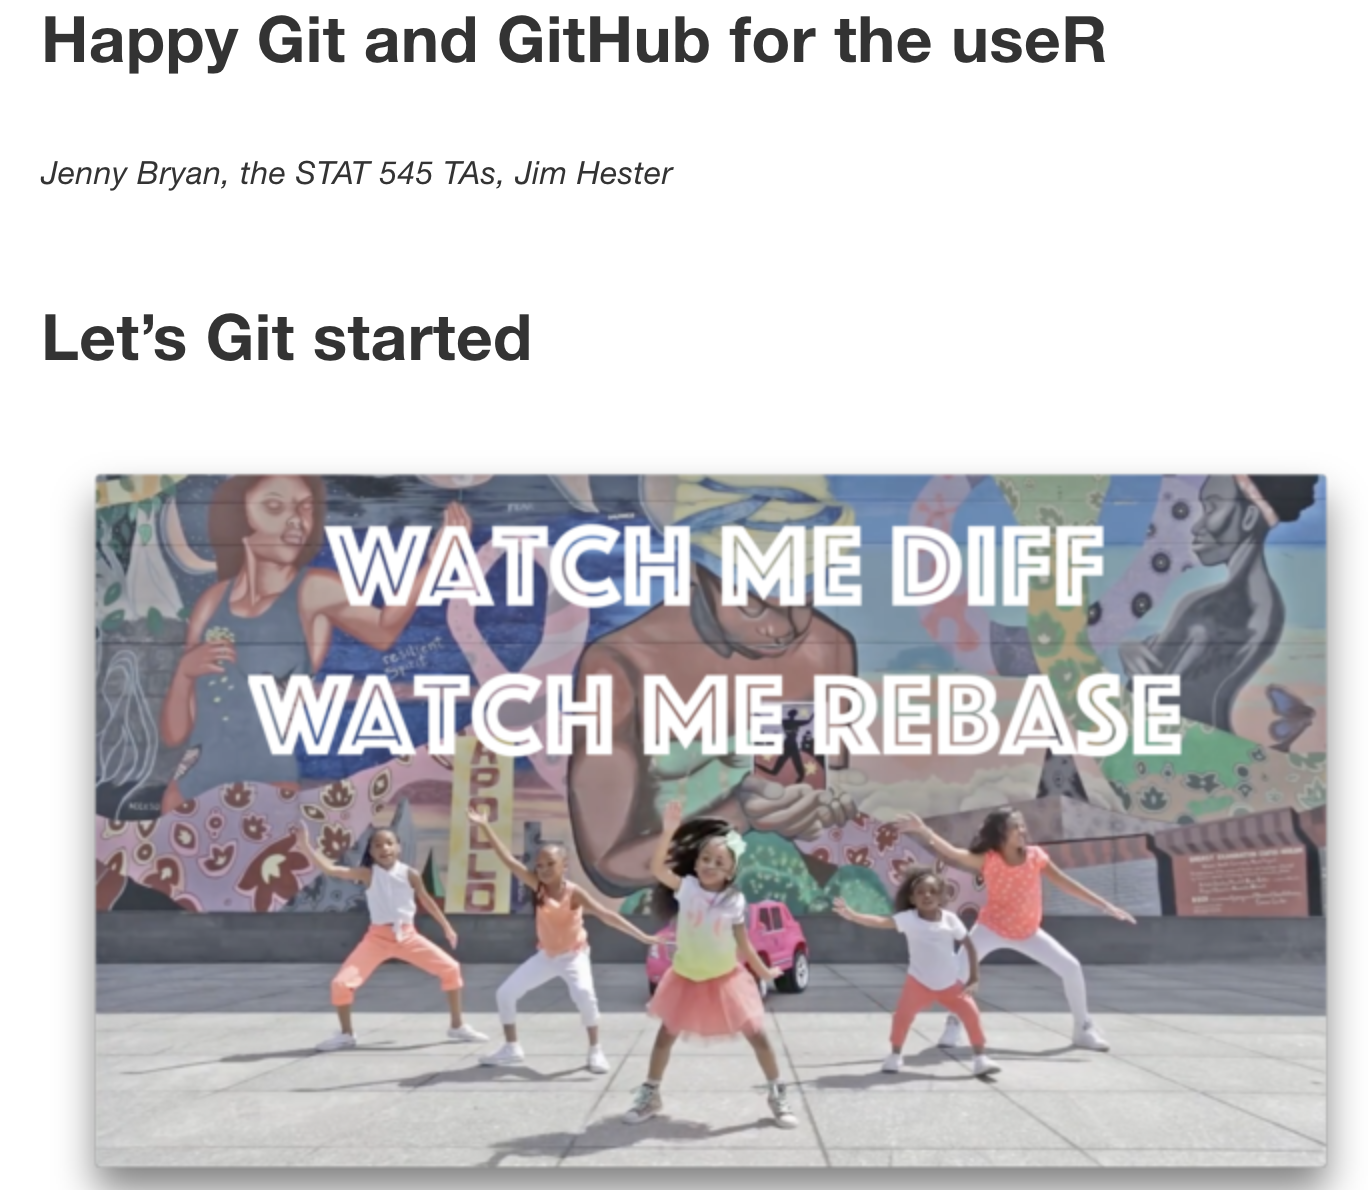
\includegraphics[width = \linewidth]{happygit.png}
\end{column}
\end{columns}
\end{frame}

\begin{frame}
\centering
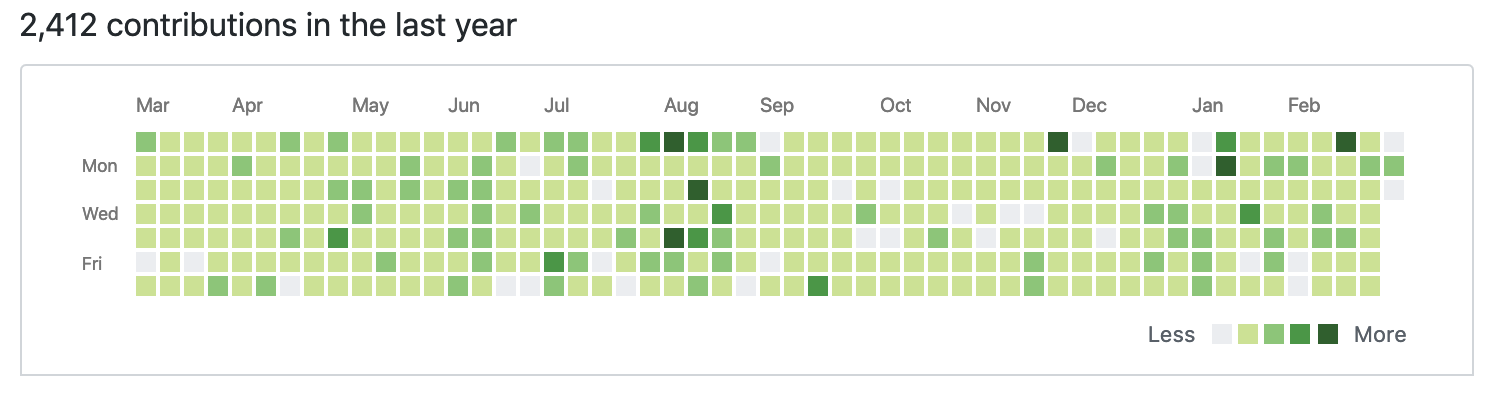
\includegraphics[width = 0.9\linewidth]{portfolio.png}
\maketitle
\end{frame}



\begin{frame}{Thanks for having me}

\begin{columns}[T]

\begin{column}{0.5\textwidth}
\bfheading{About me}
\begin{wideitemize}
\item G-4 in Government
\item American Politics, elections and representation
\item Before: Political data analytics (where I learned git from \href{https://anniejw.com/}{Annie Wang})
\end{wideitemize}\pause

\begin{wideitemize}
\item I do some software development, 
\item but most of my work is applied (``substantive'')
\end{wideitemize}
\end{column}\pause
\begin{column}{0.5\textwidth}
\bfheading{My perspective}
\begin{wideitemize}
\item Version control is mandatory for programmers (and professional data scientists)\pause
\item but does it make sense for \emph{applied} researchers who ...
\item work with datasets that are \pause ~\alert{large},\pause ~\alert{unstructured},\pause ~\alert{prone to change},\pause ~\alert{with collaborators}
\end{wideitemize}
\end{column}
\end{columns}
\end{frame}

\begin{frame}{Setting Expectations: Is it worth it?}
\begin{columns}[T]
\begin{column}{0.5\textwidth}
\bfheading{What do Gentzkow and Shapiro say?}

Definitely:
\begin{quote}
``It will probably take you a couple days to set up a repository and learn how you want to interact with [Version Control]. You will break even on that time investment within a month or two.''\footnote[frame]{Code and Data for Social Sciences: A Practioners Guide. 2014. \url{https://perma.cc/5J9D-BTD6}.  \textcolor{gray}{Although I'm not sure about learning version control in ``a couple of days'' (I certainly couldn't!), I can guarantee reading their guide in its entirety \emph{is} a time investment you'll break even on immediately.}}
\end{quote}
\end{column}
\begin{column}{0.5\textwidth}
but also see\footnote[frame]{\url{https://community.rstudio.com/t/version-control-with-google-drive/4032}}
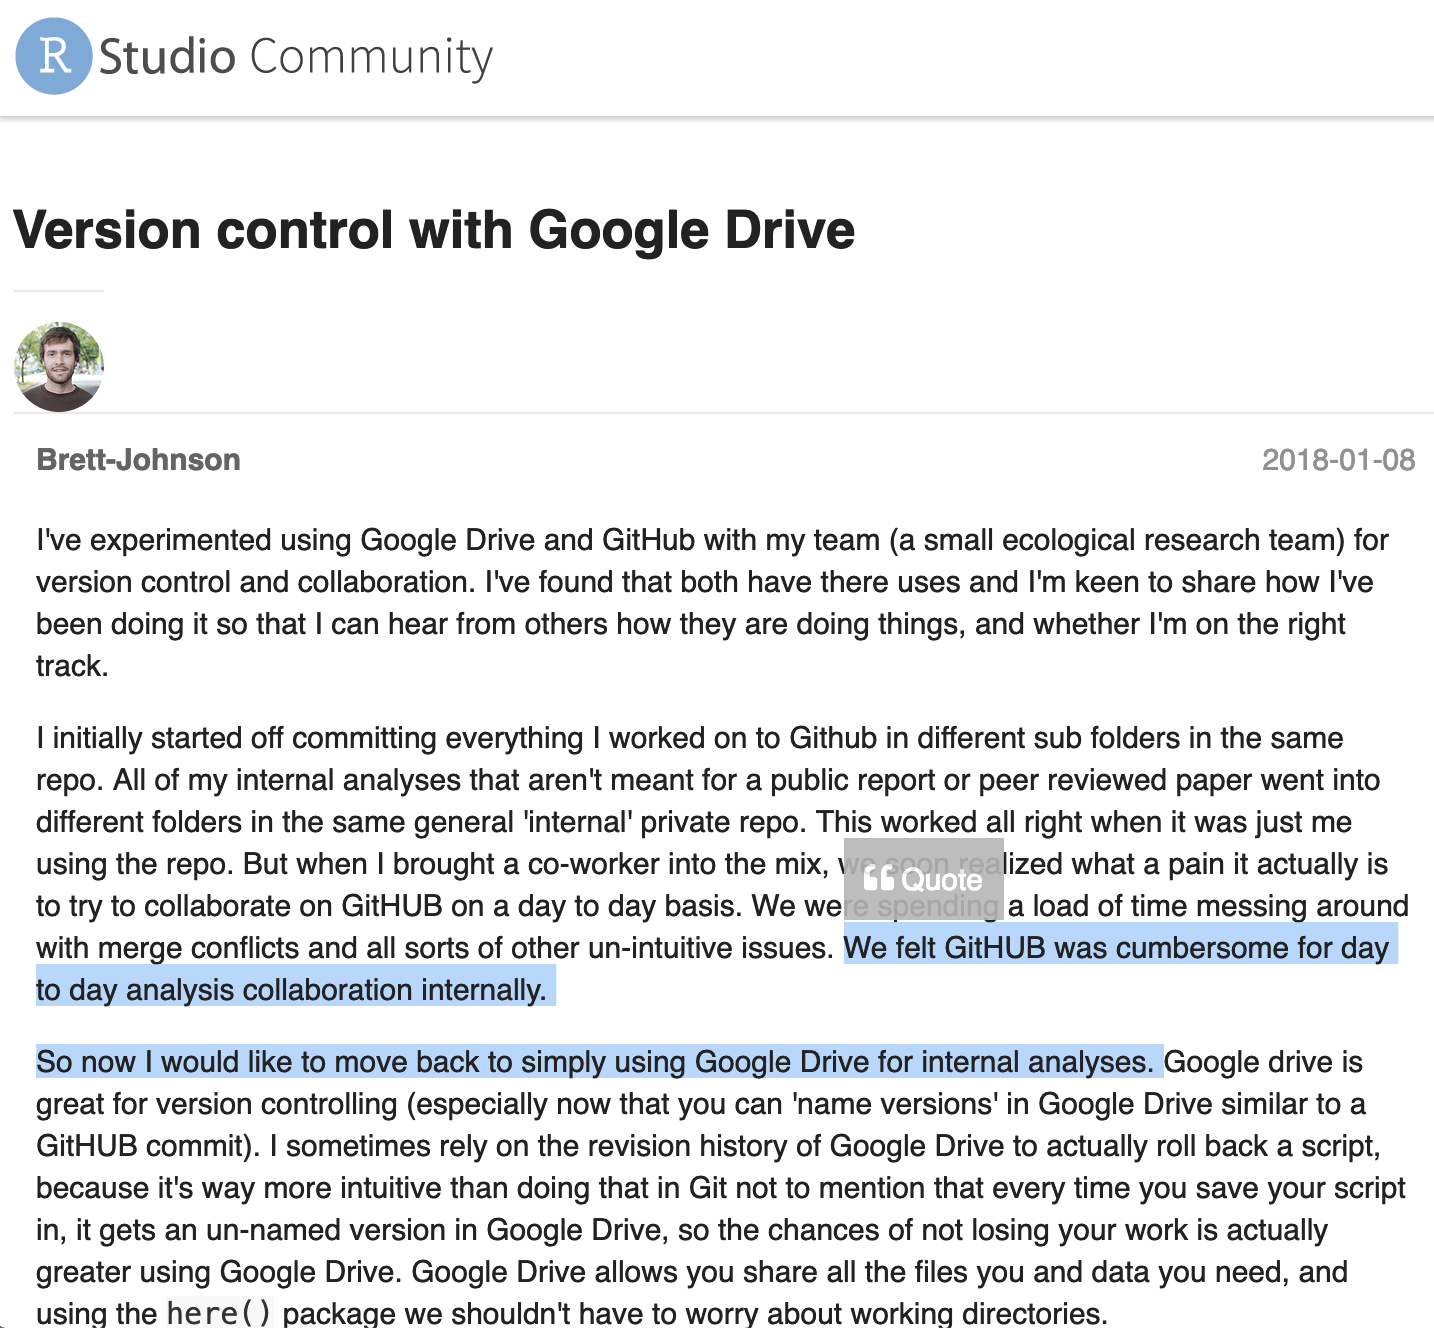
\includegraphics[width = 0.8\linewidth]{github_vs_gdrive.png}
\end{column}
\end{columns}
\end{frame}



\begin{frame}{My (recommended) setup}
\end{frame}


\begin{frame}{Terminology}
\begin{columns}[T]
\begin{column}{0.5\textwidth}
\begin{wideitemize}
\item \alert{Git} is a particular type of software for version control (Subversion is another)
\item \alert{GitHub} is an app (recently bought by Microsoft) to host git on the web (Bitbucket is another)
\item A \alert{desktop client} is an app that connects a webhost like Github to your computer and facilitates simple tasks (here I use \alert{RStudio}, there are many others)
\item A \alert{repository} is the fundamental unit of a version control, like a project folder. \pause Do not make a repository within a repository! 
\end{wideitemize}
\end{column}
\begin{column}{0.5\textwidth}
\end{column}
\end{columns}
\end{frame}

\begin{frame}{Keep Track of how your results changed}
\begin{columns}[T]
\begin{column}{0.18\textwidth}
\only<1>{\itheading{Problem: You tweak a regression specification and re-run your script, re-writing dozens of tables. You need to know how much your results changed}}
\only<2>{\itheading{You collect more data and re-run the regressions. Now how did the results change?}}
\end{column}
\begin{column}{0.82\textwidth}
\only<1>{
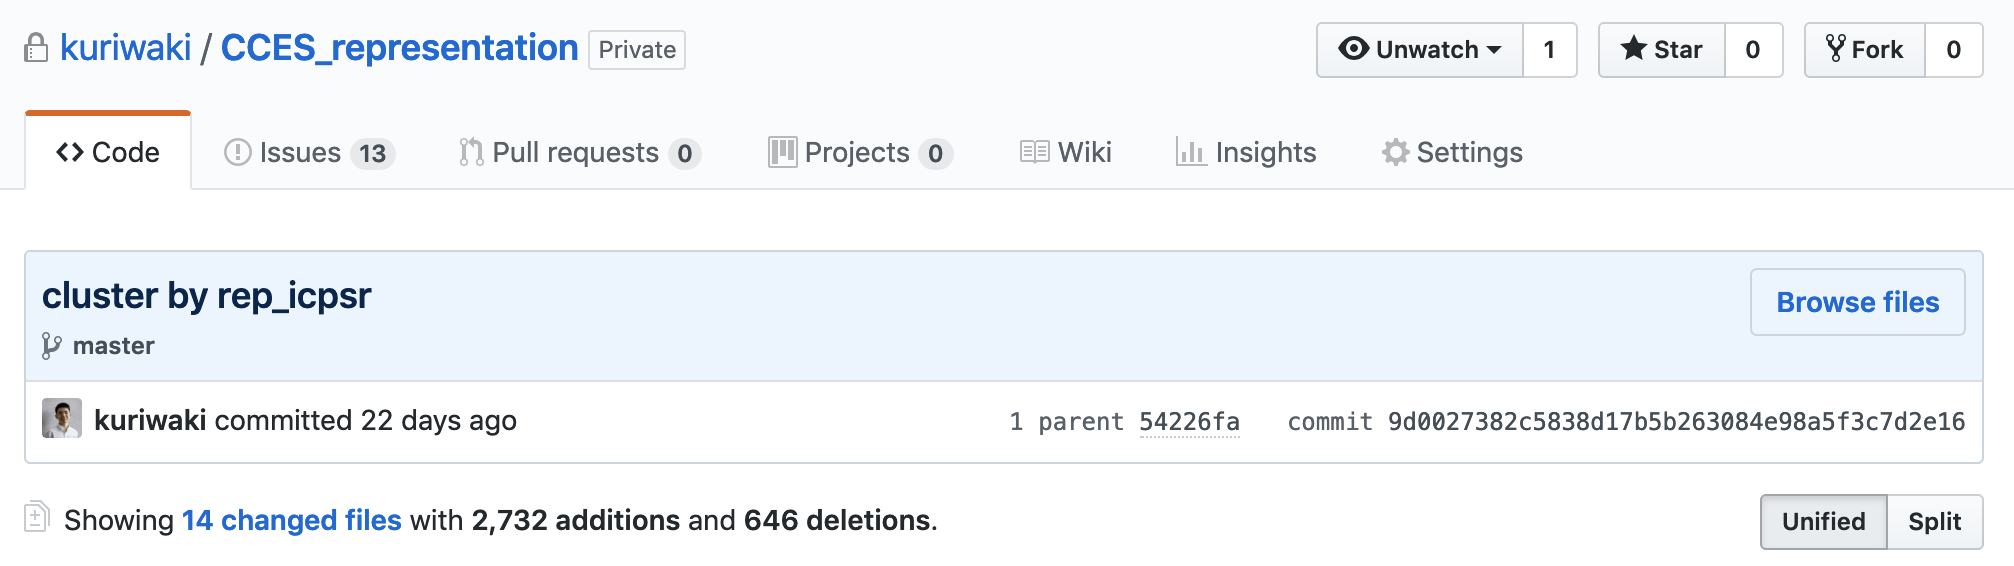
\includegraphics[width = \linewidth]{regression-diff-1.png}
...
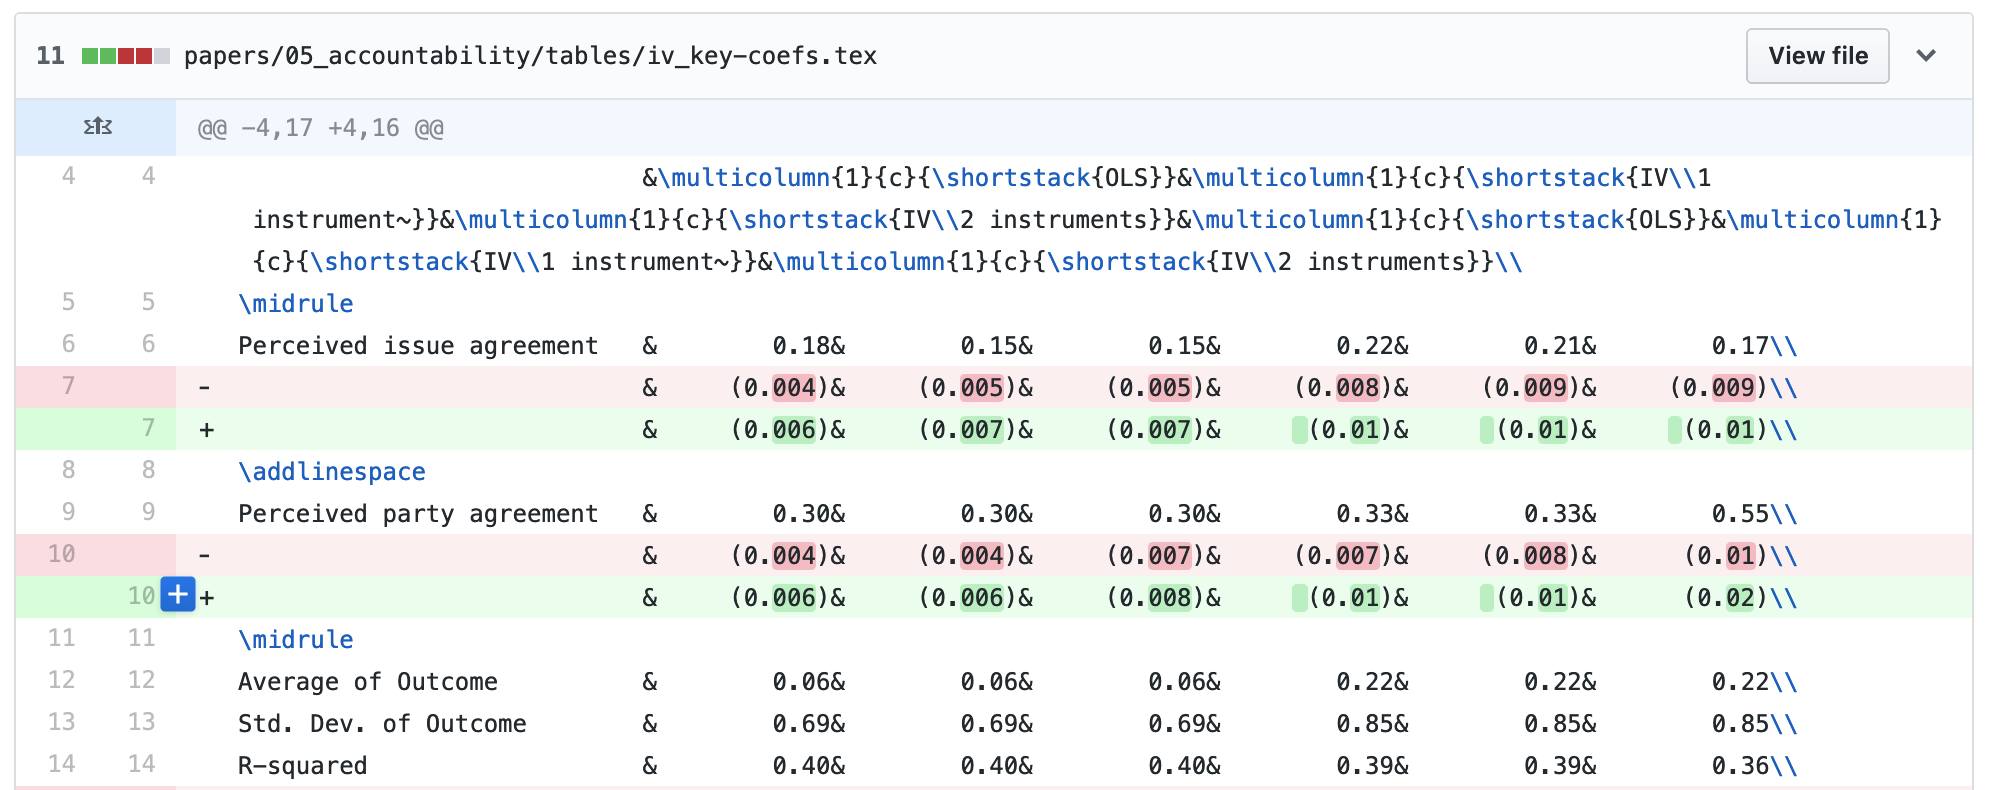
\includegraphics[width = \linewidth]{regression-diff-2.png}
}
\only<2>{

\includegraphics[width = \linewidth]{observations-diff-0.png}
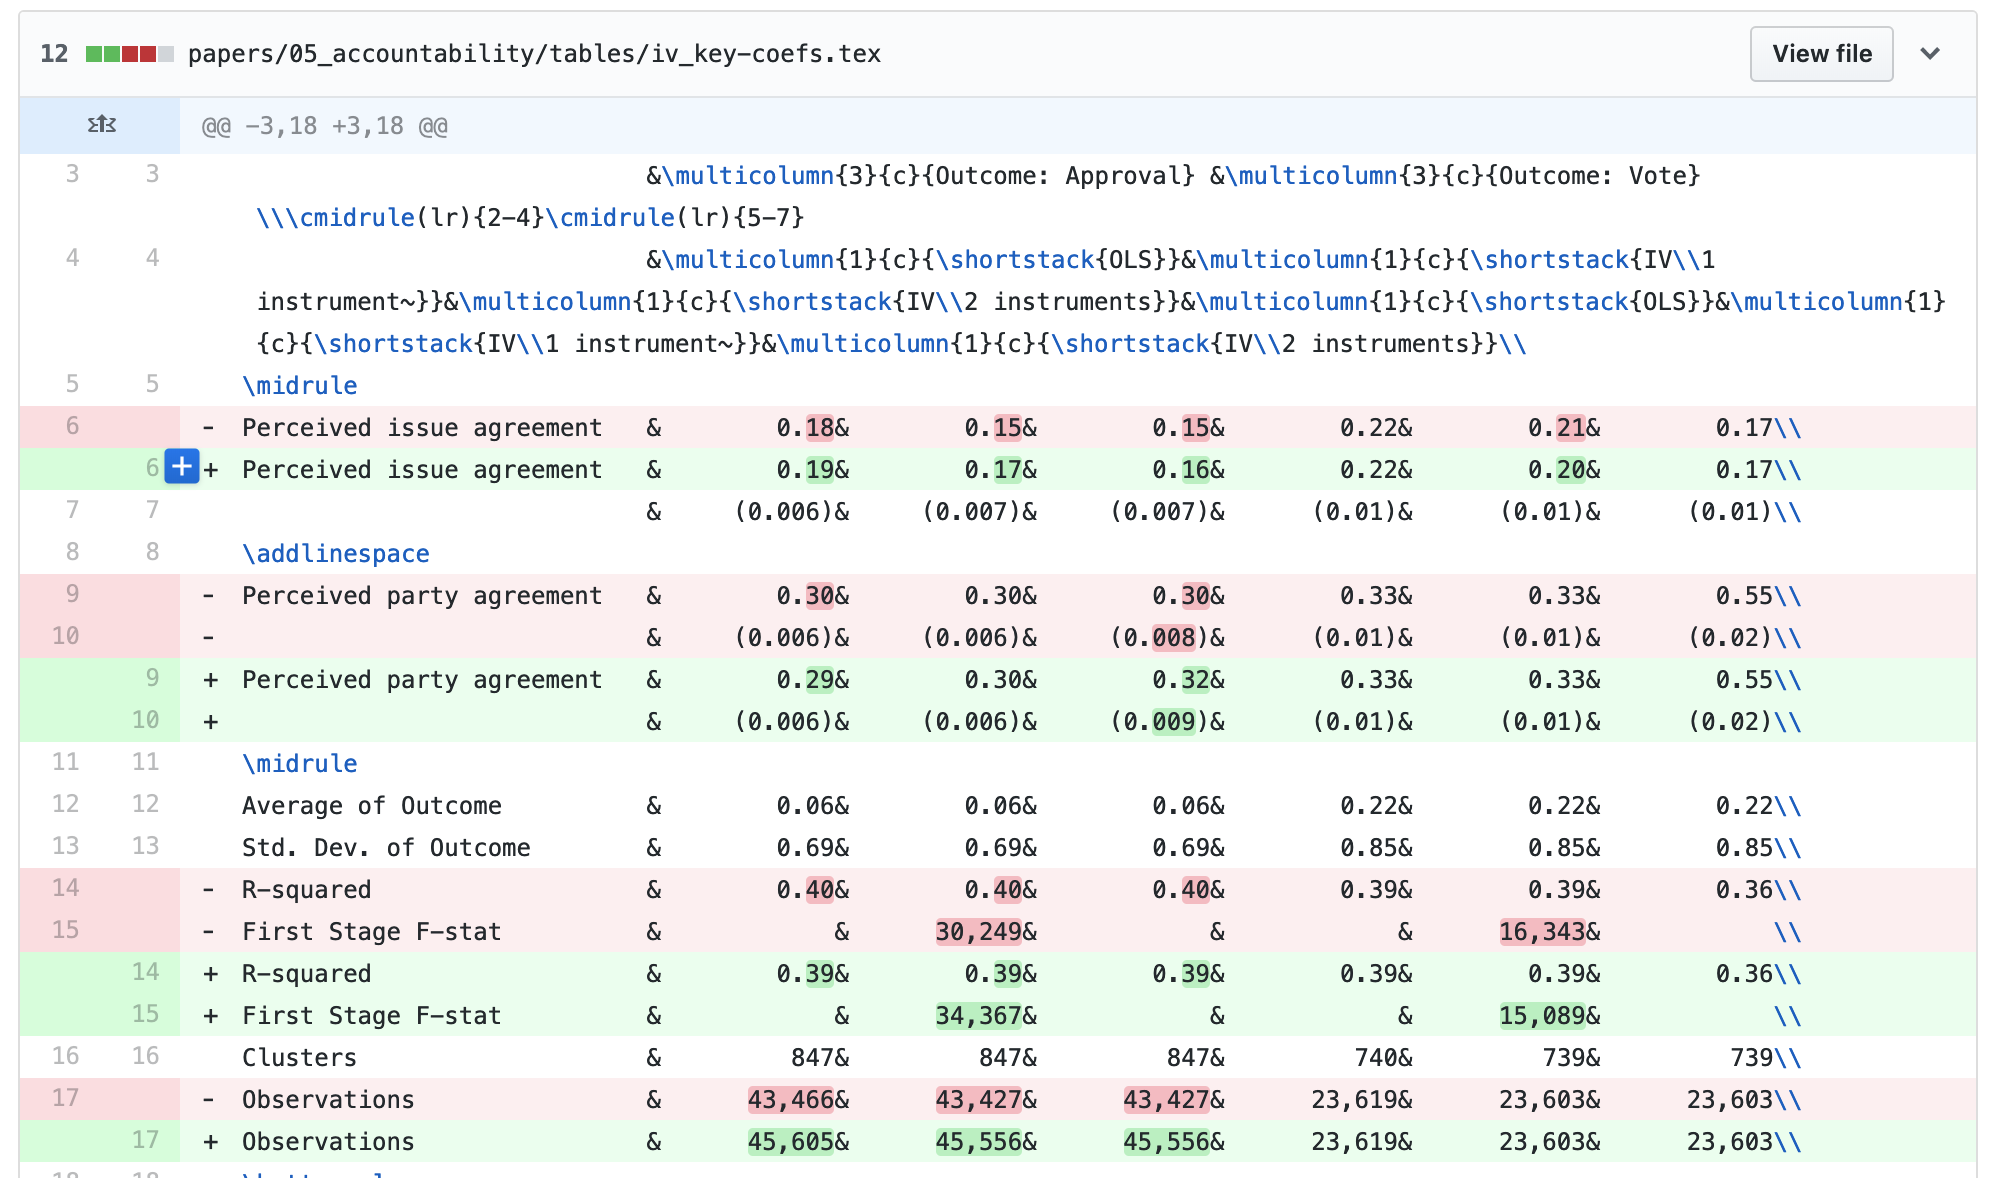
\includegraphics[width = \linewidth]{observations-diff-2.png}
}
\end{column}
\end{columns}
\end{frame}

\begin{frame}{Tracking your text changes}
\begin{columns}[T]
\begin{column}{0.4\textwidth}
\itheading{Problem: You start writing up your paper, \texttt{draft.tex}}

\begin{itemize}
\item The next day, you make a new draft. Do you overwrite?\pause
\item Or do you call it \texttt{draft\_0305.tex} ? \texttt{draft\_03052019.tex}?\pause
\item The next week, you find a single typo. Do you ``Save As'' with a new date?\pause
\item Three weeks later, you return to your paper.   Your computer indicates that the file named \texttt{draft\_0305.tex} was ``Last modified March 12, 2019''.
\end{itemize}
\end{column}
\begin{column}{0.6\textwidth}\pause
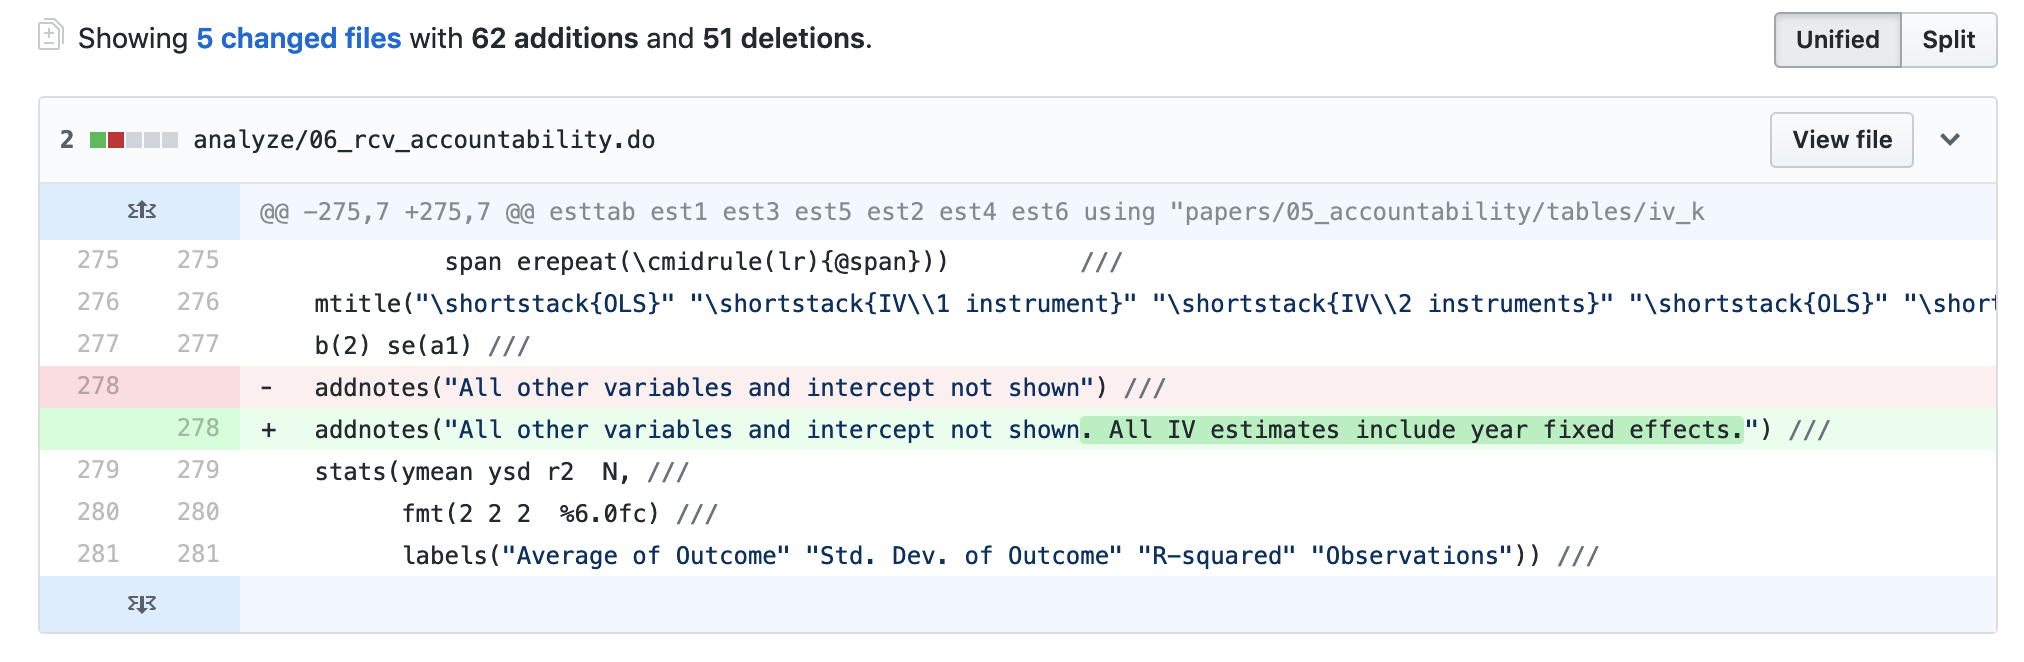
\includegraphics[width = \linewidth]{writing-diff-1.png}
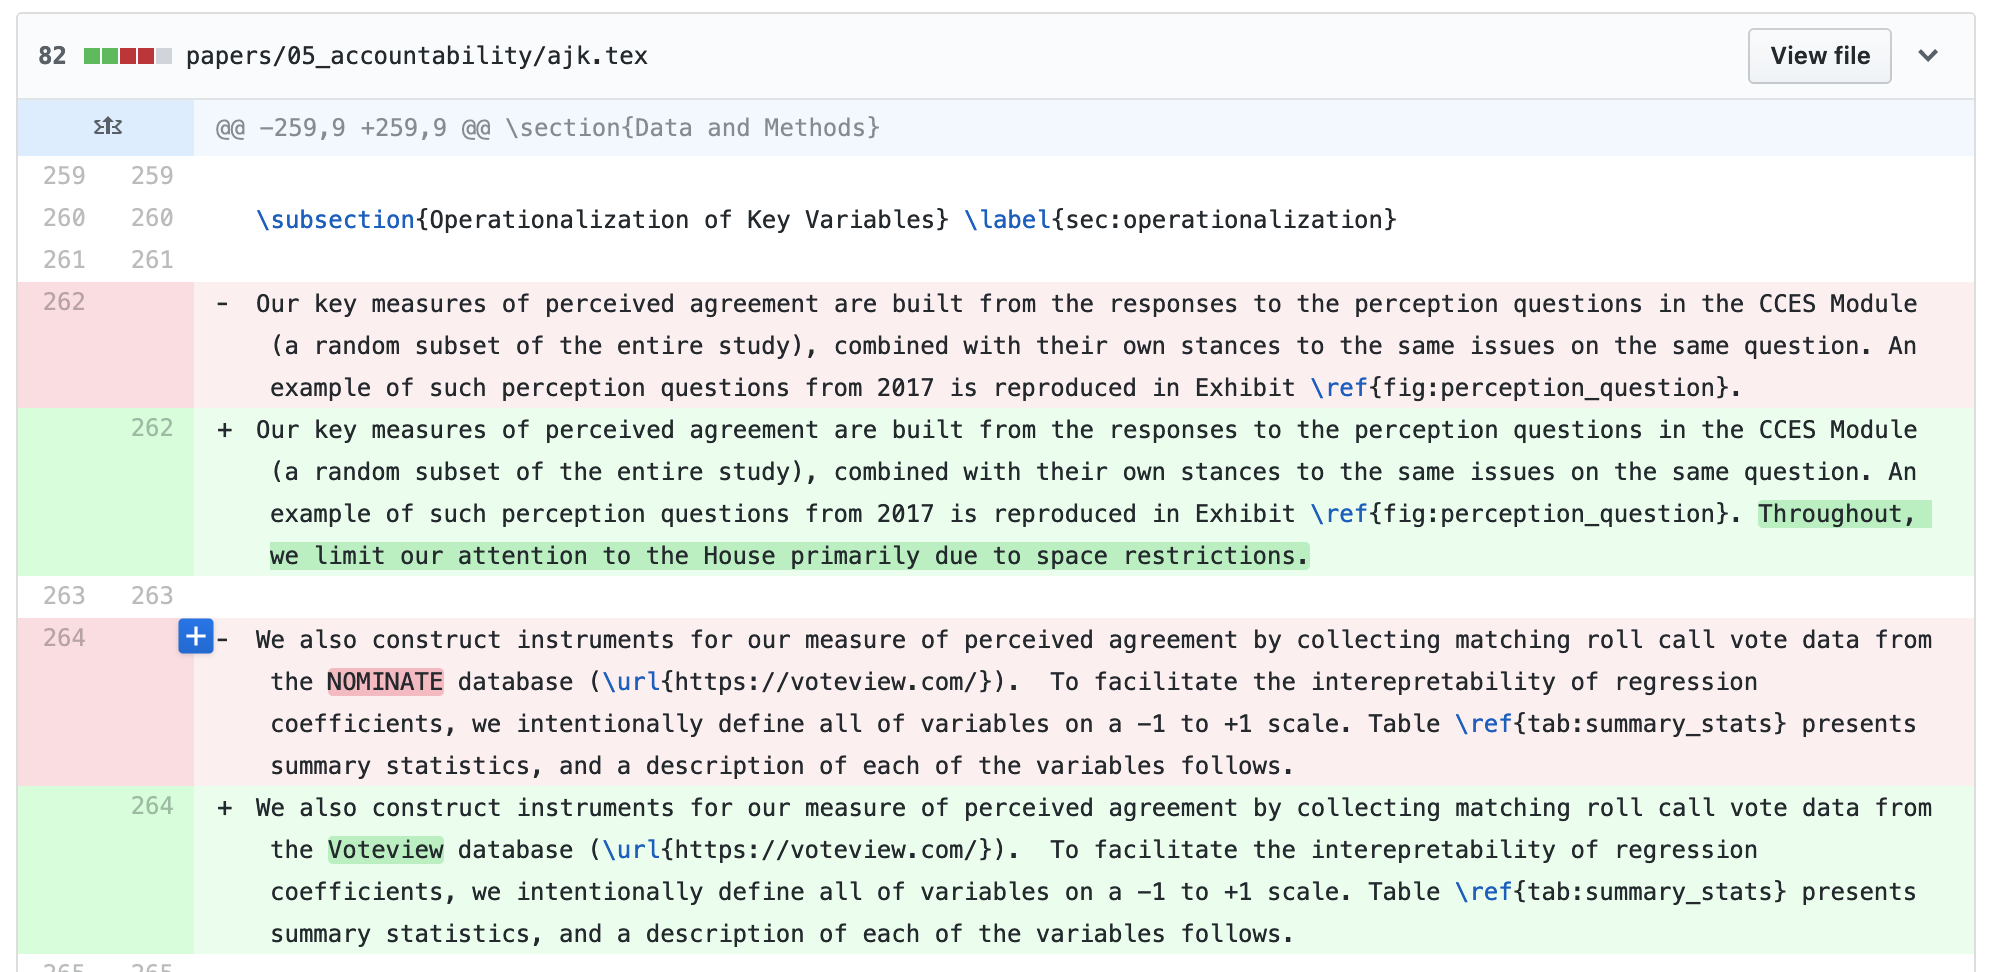
\includegraphics[width = \linewidth]{writing-diff-2.png}
\end{column}
\end{columns}
\end{frame}

\begin{frame}{And more cool stuff like}
\begin{columns}[T]
\begin{column}{0.3\textwidth}
\only<1>{\bfheading{Getting a free, customizable, add-free website}
(instead of a click-and-drag Wordpress/Squarespace website)
}
\only<2-3>{\bfheading{Work on a collaborative workbook}
(instead of needing to add people to your Dropbox)
}
\only<4>{\bfheading{Contributing to / getting the latest on actual software packages}
(Github issues is the de facto communication of open-source developers)
}
\end{column}
\begin{column}{0.7\textwidth}
\only<1> {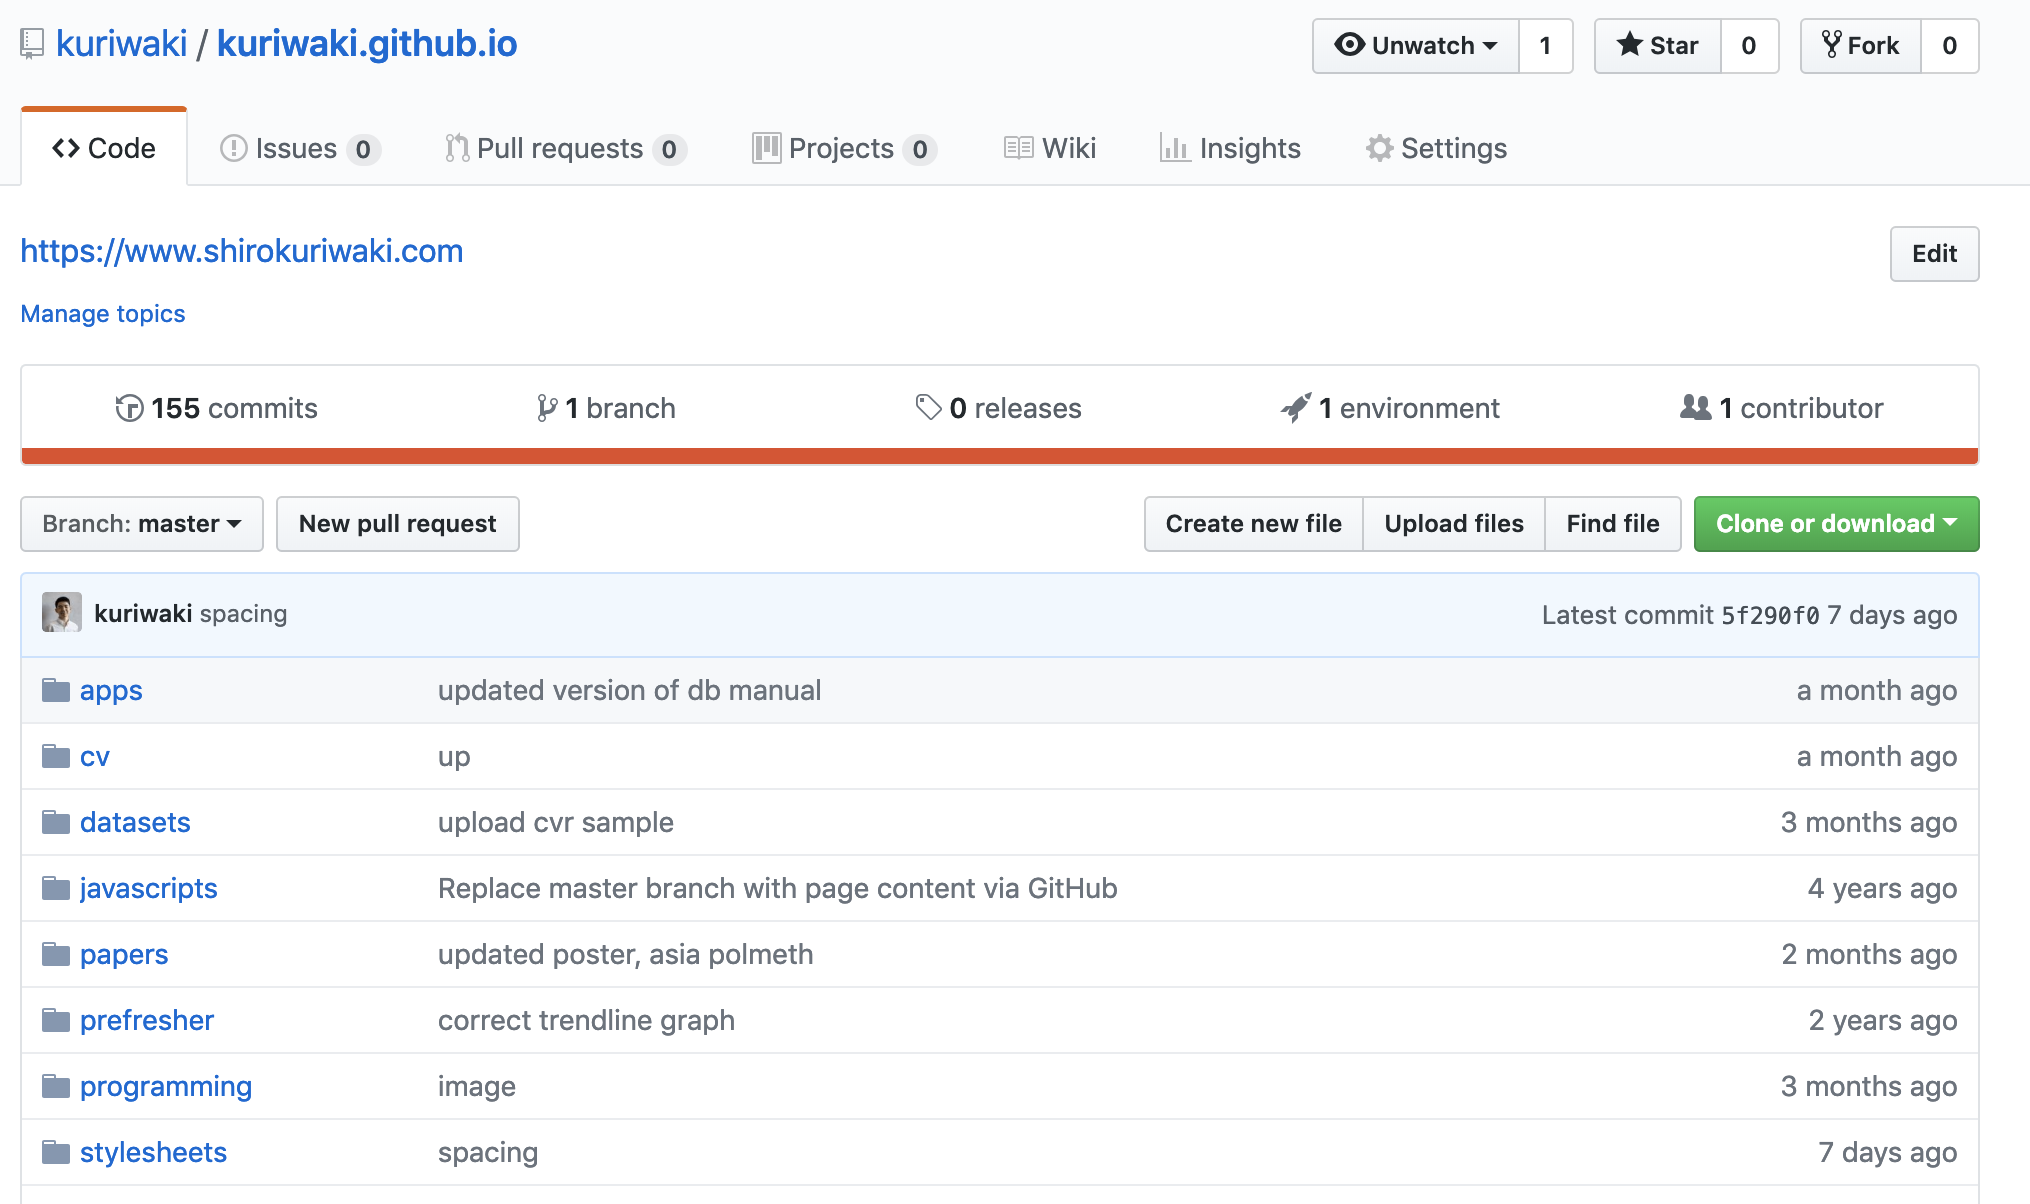
\includegraphics[width = \linewidth]{website-pages.png}}
\only<2> {
\includegraphics[width = 0.7\linewidth]{prefresher-book.png}}
\only<3> {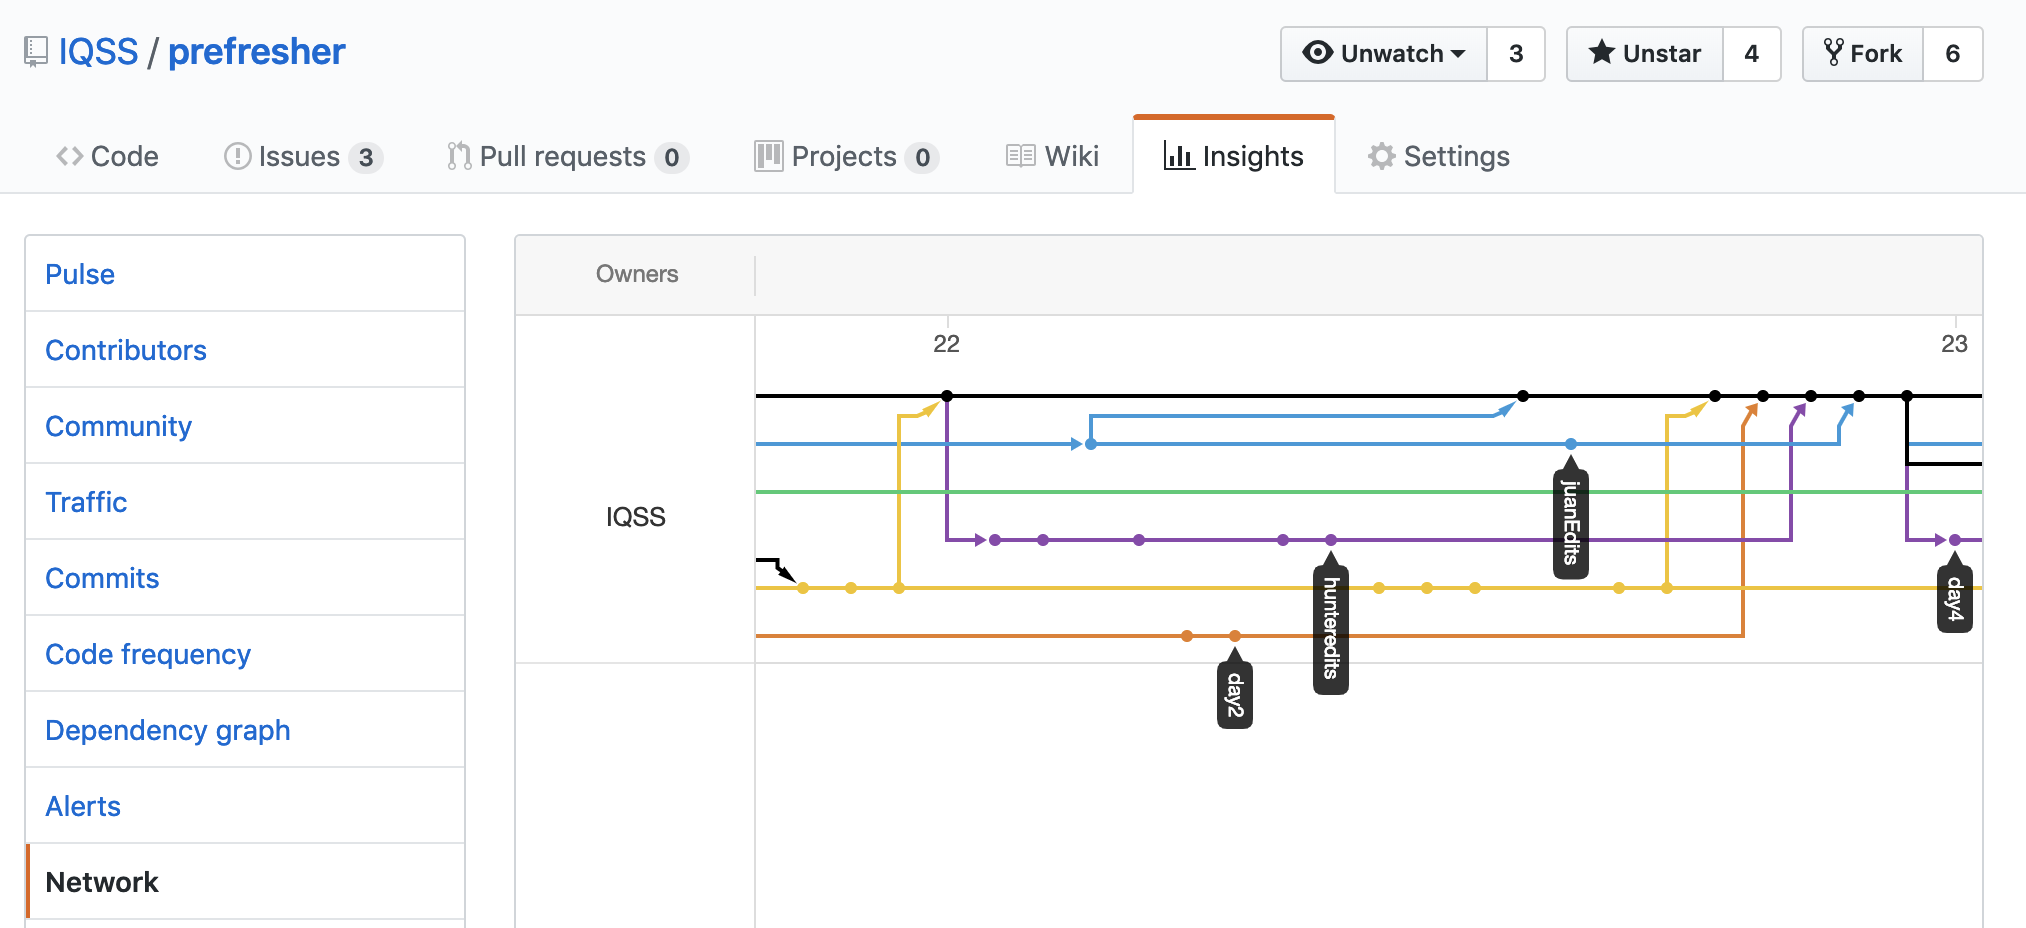
\includegraphics[width = \linewidth]{prefresher-network.png}}
\only<4> {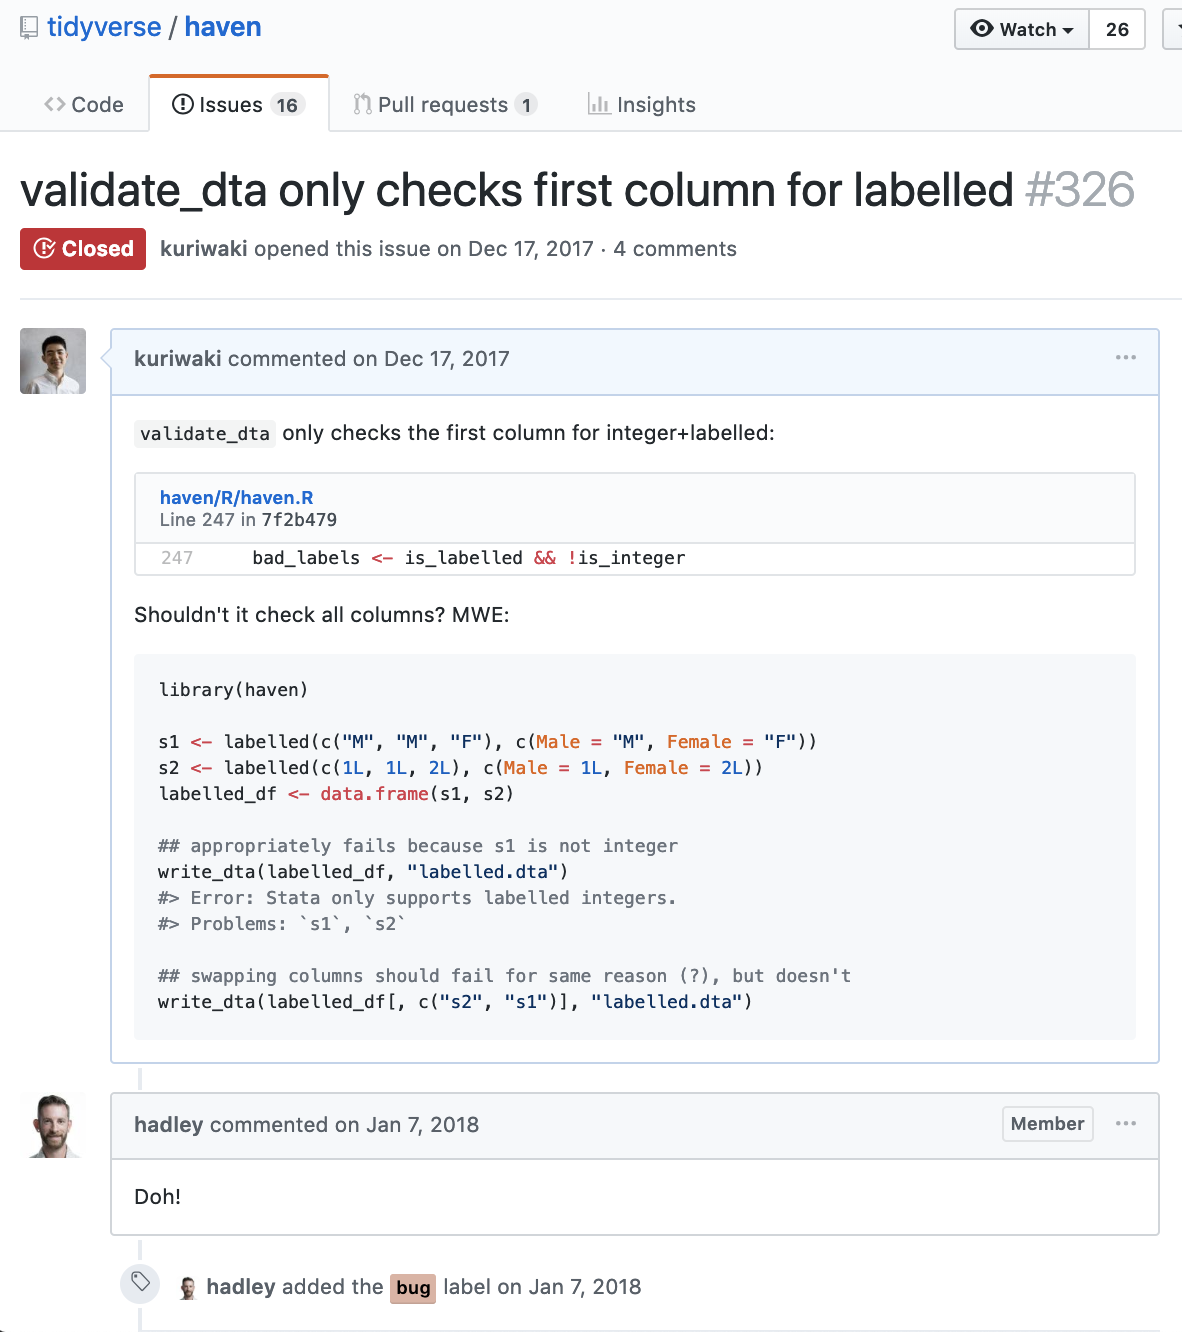
\includegraphics[width = 0.7\linewidth]{file-issues.png}}
\end{column}
\end{columns}
\end{frame}

\begin{frame}{Terminology}
\begin{columns}
\begin{column}{0.5\textwidth}
\begin{wideitemize}
\item<1-> Files increment by \alert{commit}s. The line-by-line changes from commits are called \alert{diffs}. 
\item<2-> Commits have a human-readable \alert{message}, and a serial code called a \alert{SHA} (like \code{992bb07}).
\item<3-> At least two copies of your repository exist: the \alert{local} on your computer, and a \alert{remote} (hosted on Github, with URL \code{https://github.com/user/repo.git}), \pause which has the name \alert{origin}
\item<4-> Once you make commits on your local, you \alert{push} them to your remote. (The opposite of this is a \alert{pull})
\end{wideitemize}
\end{column}
\begin{column}{0.5\textwidth}
\onslide<1->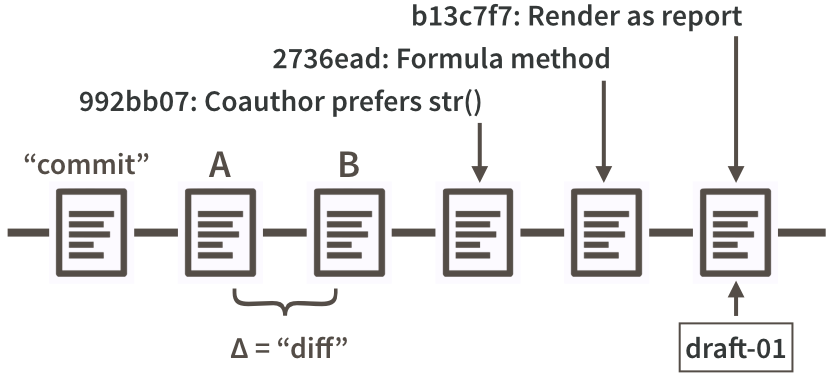
\includegraphics[width = \linewidth]{commit-diff-sha-tag.png}
\onslide<3-4>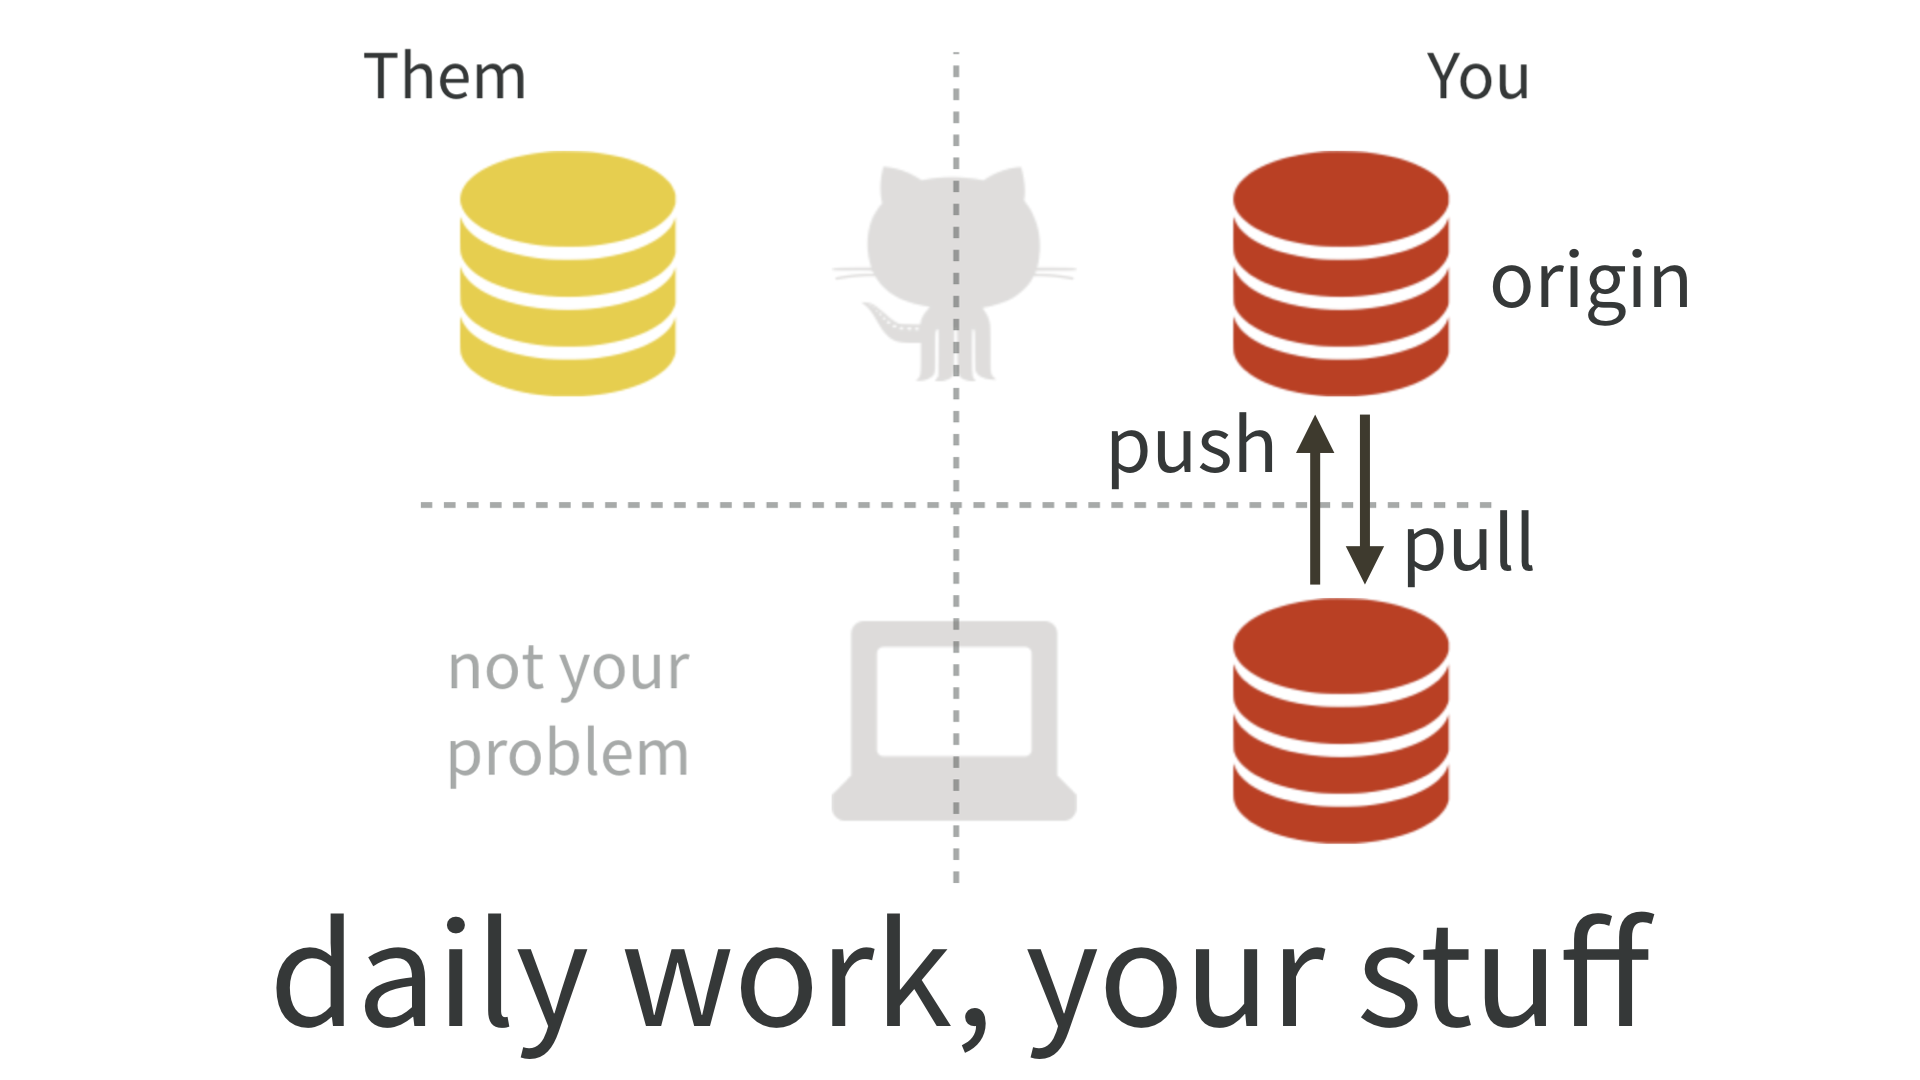
\includegraphics[width = \linewidth]{pull-push-yours.png}
\end{column}
\end{columns}
\end{frame}


% \begin{frame}{Frame}
% \begin{columns}[T]
% \begin{column}{0.5\textwidth}
% \end{column}
% \begin{column}{0.5\textwidth}
% \end{column}
% \end{columns}
% \end{frame}



\end{document}
